\section{Dataset}\label{sect:dtst}

The dataset used in this study is comprised of a population of 200 solutions, each of which is characterized by $10$ servers and $10,000$ processes. 
Each server in the dataset is defined by several attributes. 
Specifically, it has a name and a variable number of CPUs, ranging from $1$ to $10$. 
Additionally, each CPU has a variable speed, ranging from $1$ to $10$ GHz. 
The processes in the dataset are also defined by several attributes. 
Specifically, each process has a unique PID to identify it, and a length that is measured in the number of instructions required for its completion. 
The length of each process ranges from $10,000$ to $1,000,000$ instructions. 
It is worth noting that the dataset employed in this study is representative of the types of workloads commonly encountered in cloud computing environments. 
The data was collected from various sources and pre-processed to ensure consistency and accuracy. 
This dataset was specifically selected for its complexity and realistic representation of real-world cloud computing workloads. 
The use of this dataset will enable us to evaluate the effectiveness of the proposed genetic algorithm for resource allocation in cloud computing 
environments under simplified and yet realistic conditions.

% Add centered in the column the image of the dataset
%\begin{figure}[ht]
%    \centering
%    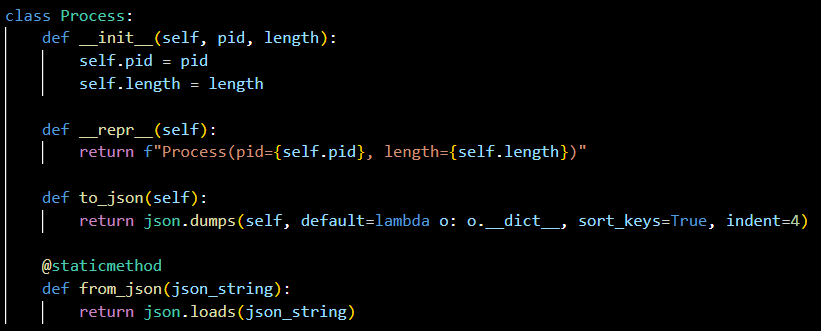
\includegraphics[width=0.5\textwidth]{./Resources/Code_Snippets/Process_Class.png}
%    \caption{The Process class.}
%    \label{fig:process}
%\end{figure}
%
%\begin{figure}[ht]
%    \centering
%    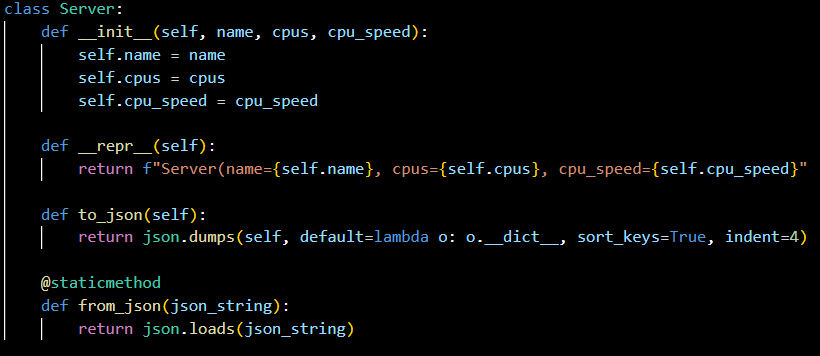
\includegraphics[width=0.5\textwidth]{./Resources/Code_Snippets/Server_Class.png}
%    \caption{The Server class.}
%    \label{fig:server}
%\end{figure}
%
%In figure~\ref{fig:process} and figure~\ref{fig:server} we can see the implementation of the Process and Server classes, which are used to represent respectively a generic Process in the
%Cloud and a Server comprising said Cloud environment.
%
%\begin{figure}[ht]
%    \centering
%    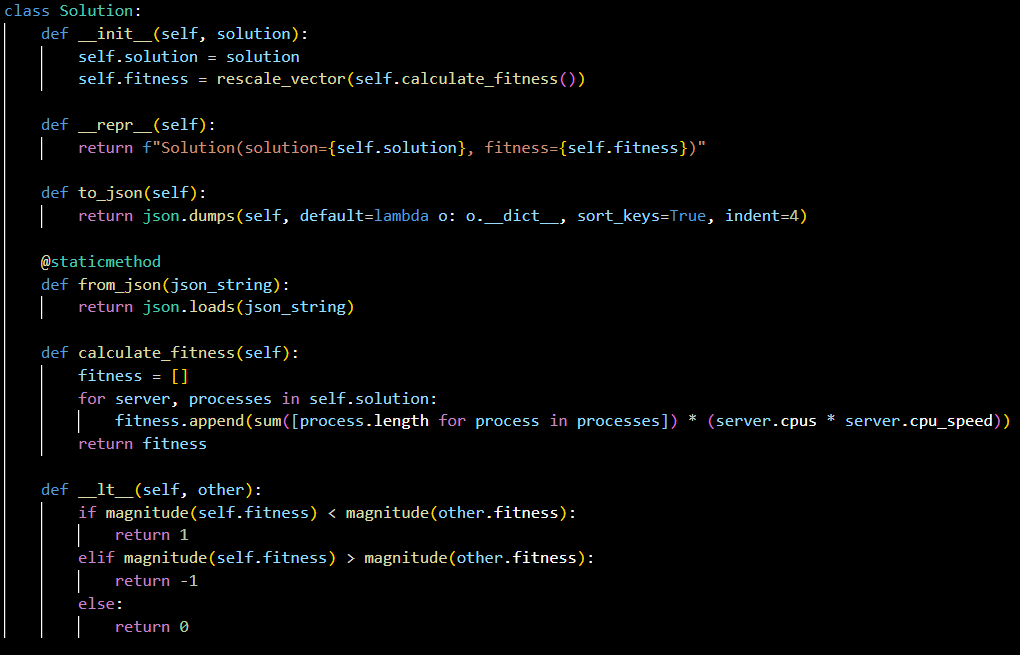
\includegraphics[width=0.5\textwidth]{./Resources/Code_Snippets/Solution_Class.png}
%    \caption{The Solution class.}
%    \label{fig:solution}
%\end{figure}
%
%The implementation shown in in figure~\ref{fig:solution} references the Solution class.

The Solution class is made of a list of tuples, each of which contains a Server and a list of Processes, and a fitness value.
The fitness value is the result of the evaluation of the solution, which is performed by the fitness function.


\newpage